\section{Agentic Tree-based Reasoning}
\label{sec:tree_based_agentic_reasoning}

%!TEX root = ../../main.tex

\begin{figure}[!t]
    \centering 
    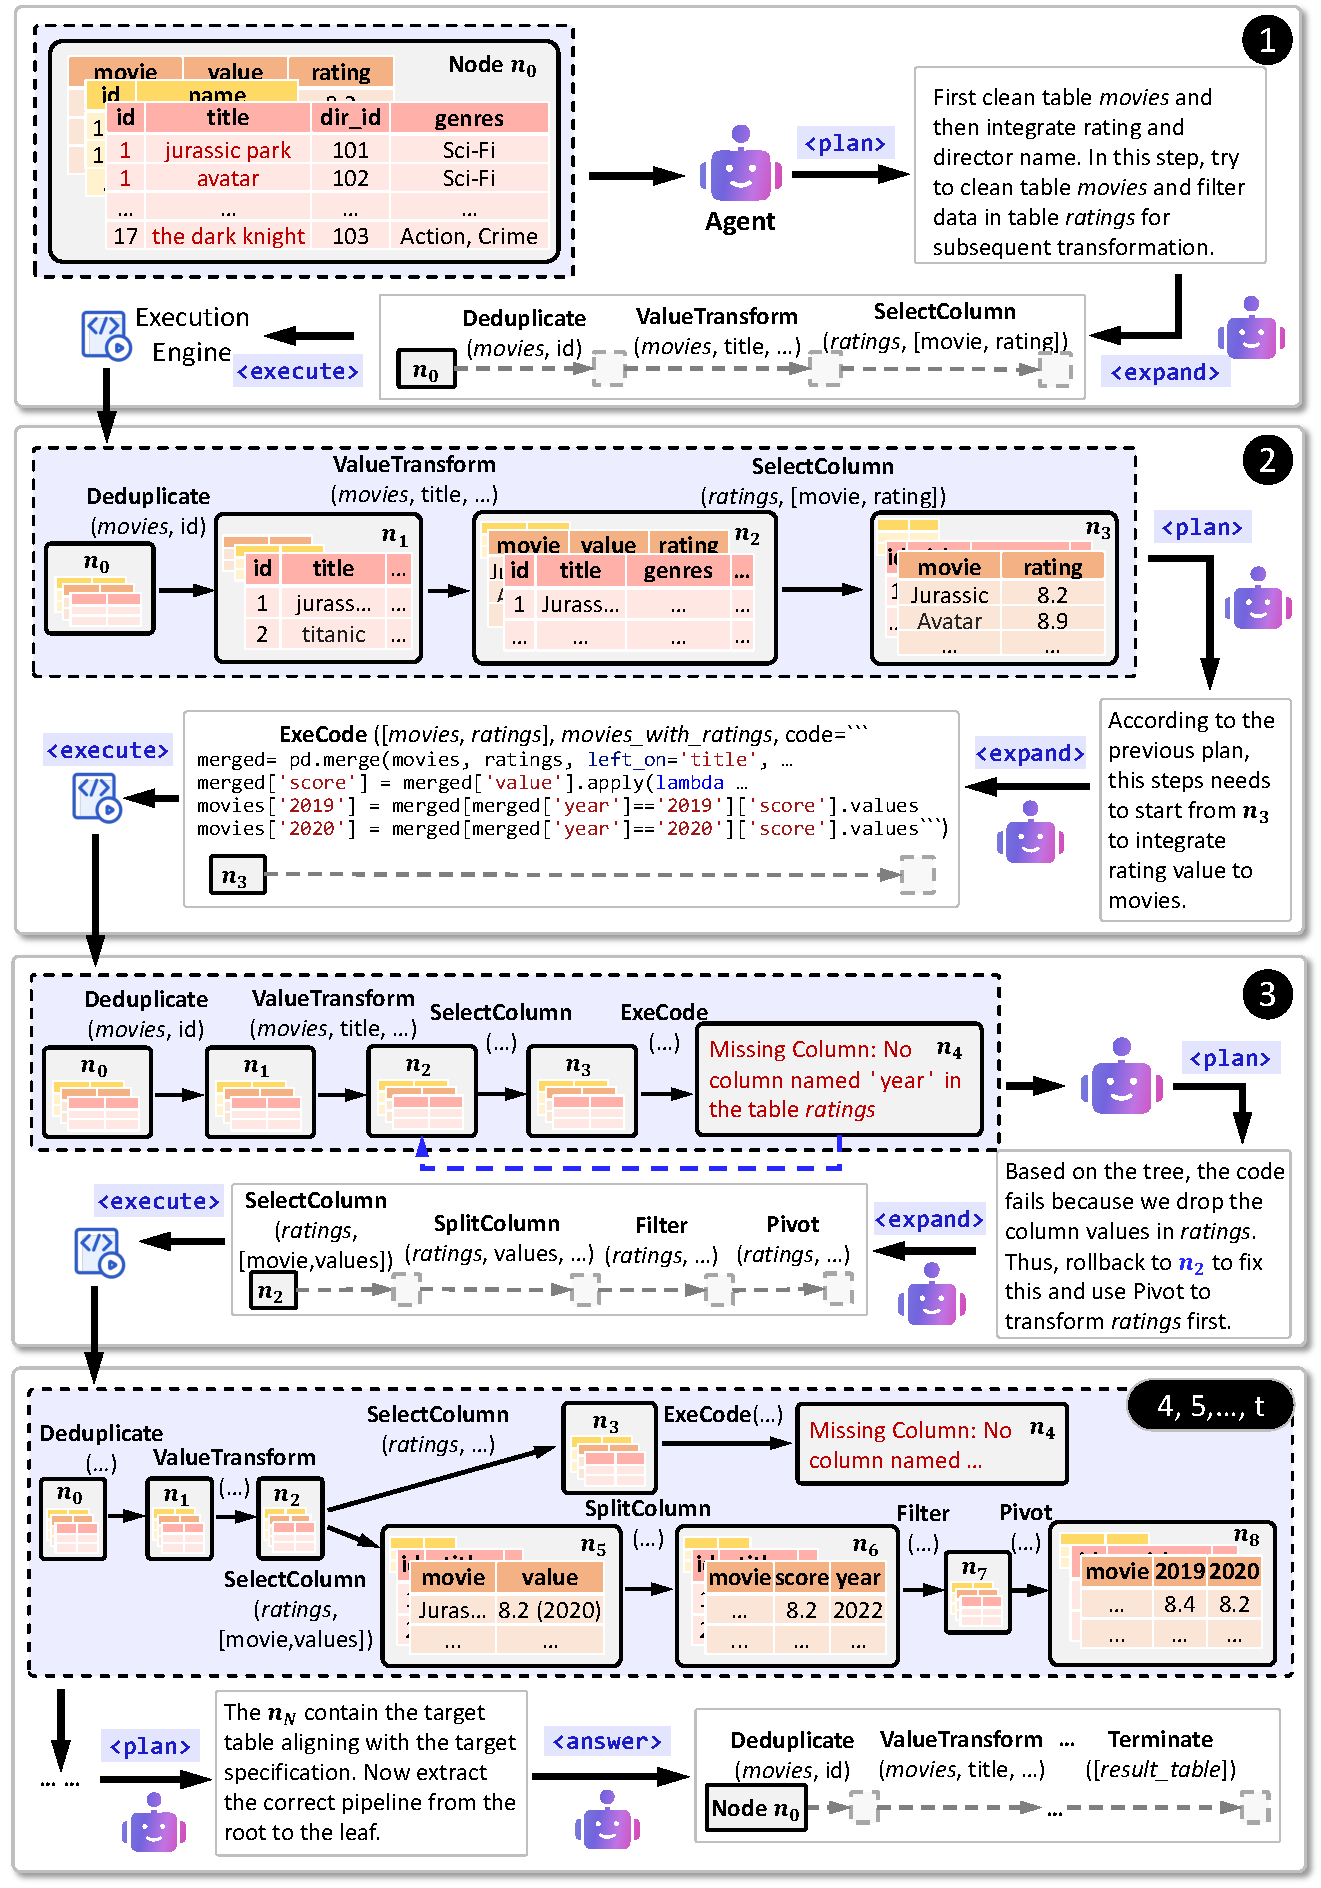
\includegraphics[width=0.99\columnwidth]{figures/fig/agentic_reasoning_example.pdf}
    \vspace{-1em}
    \caption{An example of tree-based agentic reasoning.
    }
    \label{fig:agentic_reasoning_example}
     \vspace{-1.5em}
\end{figure}

As established in Section~\ref{subsec:agentic_reasoning_preliminary}, the sequential nature of ADP can be naturally modeled as an agentic reasoning task.
However, directly applying standard frameworks like linear ReAct-style reasoning~\cite{yao2023react} for agentic reasoning introduces a critical limitation: \textit{irreversibility}.
In such naive implementations, the state is restricted to the \textit{current} data snapshot (i.e., $x_t = \mathcal{D}_t$), forcing the agent to progress linearly ($x_{t+1}=\mathcal{P}(x_t, o_t)$).
While effective for general tasks, this linear topology is insufficient for data preparation. This is because many operators (e.g., filtering or aggregation) cause \textit{irreversible information loss}, meaning the original data cannot be recovered from the transformed state.

\begin{example}
%
Consider the task in Figure~\ref{fig:introduction_example}, where the goal is to report each director's average rating by \textit{single} genre for years 2019 and 2020.
A crucial step is to apply \texttt{Explode} on the \texttt{genres} column, since a movie can belong to multiple genres (e.g., ``{Sci-Fi, Action}'').
If the agent overlooks \texttt{Explode} and directly performs aggregation (e.g., \texttt{GroupBy} on \texttt{director\_name} and \texttt{genres}), the aggregation treats a multi-genre cell as one atomic category.
Consequently, the computed performance metrics become incorrect, because ratings that should be attributed to \texttt{Sci-Fi} and \texttt{Action} separately are instead merged into an artificial combined label.
At this point, the error is hard to recover in a purely linear ReAct-style rollout, because the current state has already discarded the per-genre attribution needed for correct aggregation.
Since the agent only retains the latest transformed snapshot, it cannot return to the pre-aggregation table to insert \texttt{Explode}, making the correct target table unreachable from the wrong state.
\end{example}

To address this, we propose an \textbf{Agentic Tree-based Reasoning} framework. By maintaining the full history of data states, execution results, and reasoning plans as a \textit{State Transition Tree}, our framework empowers the agent to perceive the global decision space and actively backtrack from such dead-ends to explore alternative valid paths.

\subsection{Definition}

We instantiate the agentic formulation to explicitly address the challenges of irreversibility and error propagation.

\stitle{State ($\mathcal{X}$).} 
To enable global planning and backtracking, we define the state space $\mathcal{X}$ not as single data snapshots, but as the set of all possible \textit{State Transition Trees} $\mathcal{T} = (\mathcal{N}, \mathcal{E})$. 

\begin{itemize}[leftmargin=1em]
    \item {Node ($\mathcal{N}$)}. Each node $n \in \mathcal{N}$ is defined as $(\mathcal{D}_n, \eta_n, \psi_n)$, capturing the snapshot task state: (1) {Physical State} $(\mathcal{D}_n, \eta_n)$: $\mathcal{D}_n$ denotes the data environment consisting of source tables and intermediate tables, and $\eta_n$ represents the execution feedback (e.g., error tracebacks, or sample rows) from the previous operator. (2) {Cognitive State} $(\psi_n)$: $\psi_n$ represents the reasoning plan of the agent that justifies the transition to this node. By persisting thoughts in the tree, the agent can later review its own reasoning history to identify logical errors.
    \item {Edge ($\mathcal{E}$).} A directed edge $e = (o(n^{(i)}) \rightarrow n^{(j)}) \in \mathcal{E}$ represents a parameterized operator $o$ that transforms the node $n_i$ into $n_j$, driven by the cognitive state $\psi_i$. 
\end{itemize}

\stitle{Action Space ($\mathcal{A}$).}
We define a set of atomic actions that allow the agent to navigate this tree non-linearly, effectively solving the irreversibility problem. The actions defined here (e.g., \texttt{<expand}) is different from data preparation operators (e.g., \texttt{GroupBy})

\begin{itemize}[leftmargin=1em]
\item \texttt{<analyze} ($\mathcal{T}, \mathcal{S} \to \psi_{new}$): The agent inspects the current State Transition Tree $\mathcal{T}$ and the target specification $\mathcal{S}$ to generate a new reasoning plan $\psi_{new}$ for this step. This plan determines the next transition strategy, such as extending the current path, backtracking to a previous node to resolve an error, or halting.
\item \texttt{<expand} ($n_{parent}, \psi_{new} \to \Delta \Pi$): Based on the plan, the agent identifies a target parent node $n_{parent} \in \mathcal{N}$ and generates a candidate sequence of operators $\Delta \Pi$. This step translates the high-level reasoning plan into concrete, executable operators. To ensure robust node selection, we constraint the LLM to regenerates the operator from scratch. Then we employ a prefix-matching strategy to select the first unmatched operator $o^*$. The node before $o^*$ is the selected node $n_{parent}$. This design avoids the ambiguity of numerical indexing~\cite{wallace2019nlp} and reduce the complexity of this action.
\item \texttt{<terminate} ($\mathcal{T}, \mathcal{S} \to \Pi$): Triggered when the agent confirms that a leaf node satisfies the target specification $\mathcal{S}$. It extracts a path from the root to this leaf as the final solution $\Pi$.
\end{itemize}

\stitle{Environment Transition ($\mathcal{P}$).} 
The transition function $\mathcal{P}$ updates the tree structure $\mathcal{T}$ by materializing the operator sequence generated by the \texttt{<expand} action. 
Formally, given a target parent node $n_{parent}$, the associated reasoning plan $\psi_{new}$, and the expanded candidate operators $\Delta \Pi = (o_1, \dots, o_k)$, the environment performs a sequential execution.
We initialize the starting state as $n^{(0)} = n_{parent}$. For each step $j \in [1, k]$, the system applies operator $o_j$ to the data environment of the predecessor node:
$$
(\mathcal{D}^{(j)}, \eta^{(j)}) = \mathcal{F}_{op}(\mathcal{D}^{(j-1)}, o_j)
$$
where $\mathcal{F}_{op}$ refers to the operator execution engine. It executes the operator $o_j$ and captures the feedback (e.g., sample rows or error tracebacks). 
A new node $n^{(j)} = (\mathcal{D}^{(j)}, \eta^{(j)}, \psi_{new})$ is created and attached via the edge $o_j(n^{(j-1)}) \rightarrow n^{(j)}$.
Crucially, this sequential process possesses an \textit{early-stop mechanism}: if $\eta^{(j)}$ contains an execution exception, the expansion halts immediately, and subsequent operators $(o_{j+1}, \dots, o_k)$ are discarded. Finally, the updated tree $\mathcal{T}_{new}$ with new added nodes is returned.

\subsection{Reasoning Process}
\label{subsec:reasoning_algo}

Given an ADP task $(\mathcal{D}, \mathcal{S})$.
The initial state is the root tree $\mathcal{T}_0 = (\mathcal{N}_0, \mathcal{E}_0) \; \text{with} \; \mathcal{N}_0 = \{n_0\}, \; n_0 = (\mathcal{D}, \emptyset, \emptyset).$
At each decision step $t \in \{1,\dots,T\},$ the agent generates a structured action $a_t \in \{\texttt{<analyze}, \texttt{<expand}, \texttt{<terminate}\}$ conditioned on the current tree:
$
a_t \sim \pi_\theta(\cdot \mid \mathcal{T}_{t-1}, \mathcal{S}).
$
If $a_t = \texttt{<expand}$, the environment executes a candidate operator sequence and updates the tree via the early-stop mechanism, returning the new state $\mathcal{T}_t$ with execution feedback and reasoning plan stored in the created node(s).
If $a_t = \texttt{<terminate}$, the process stops and extracts the final pipeline $\Pi$ from a selected root-to-leaf path.

\stitle{An illustrative example.}
Figure~\ref{fig:agentic_reasoning_example} depicts a portion of reasoning trajectory for the task in Figure~\ref{fig:introduction_example}.
The process begins with the root $n_0=(\mathcal{D}_{init}, \emptyset, \emptyset)$.
In the first iteration, the agent uses \texttt{<analyze} to formulate a reasoning plan $\psi_1$: ``Prioritize cleaning the \textit{movies} table.'' It then triggers \texttt{<expand} to generate \texttt{Deduplicate} and \texttt{Standardize} operators. The environment executes these, creating nodes $n_1, n_2$, where feedback $\eta$ contains sample rows for verification.
Next, the agent attempts to process the \textit{ratings} table (plan $\psi_2$). However, the generated \texttt{ExeCode} operator fails due to a syntax error. The environment transitions to a failure node $n_3$, where $\eta_3$ contains the {exception traceback}.
Observing this failure in the next \texttt{<analyze} step, the agent decides to \textbf{backtrack}. It selects the valid parent $n_2$ and proposes an alternative strategy $\psi_4$ (e.g., using \texttt{Pivot}). This corrective branch leads to a node $n_6$ containing a updated table \textit{ratings} ready for joining. 
Finally, after $t$ steps, the agent verifies the leaf node against $\mathcal{S}$ and invokes \texttt{<terminate} to extract the final operator pipeline.

\stitle{Comparison with MCTS.}
While our framework shares structural similarities with Monte Carlo Tree Search (MCTS), it diverges fundamentally in state representation and feedback mechanisms. First, {Holistic vs. Snapshot States.} Existing MCTS-based data agents~\cite{ge2025monteprep} typically model states strictly as data snapshots. In contrast, our node definition $(\mathcal{D}, \eta, \psi)$ couples the data with {execution feedback} and {reasoning plan}. This allows the agent to distinguish between data-level issues and logic-level misconceptions. Second, {Semantic vs. Scalar Feedback.} MCTS relies on coarse-grained scalar rewards (e.g., success/fail) to guide search. Conversely, our framework harnesses {semantic feedback} from execution logs. By analyzing specific error messages in $\eta$, the agent performs targeted debugging rather than stochastic trial-and-error, significantly pruning the search space of invalid operators.
% reasoning plan
